%%=====================================================================================
%%
%%       Filename:  articulo.tex
%%
%%    Description:  Artículo
%%
%%        Version:  1.0
%%        Created:  10/03/2018
%%       Revision:  none
%%
%%         Author:  Herbert Arias (dayanqwe123@gmail.com), 
%%   Organization:  
%%      Copyright:  Copyright (c) 2018, Herbert Arias.
%%
%%          Notes:  
%%
%%=====================================================================================

\documentclass[twocolumns,a4paper]{IEEEtran}
\usepackage{graphicx}
\usepackage{amsmath}
\usepackage{authblk}
\usepackage[spanish]{babel}
\usepackage{blindtext}
\usepackage[utf8]{inputenc}
\usepackage{hyperref} 
\hypersetup{hidelinks}
\usepackage{csquotes} 
\usepackage[style=ieee]{biblatex} 
\bibliography{Bibliography.bib}

\graphicspath{{./pictures/}}

%%\title{Un breve recorrido por las tecnologías de Desarrollo Web en el 2018 }
\title{Rutas para el aprendizaje de tecnologías del desarrollo Web en la actualidad}

\author[1]{Herbert Brice Arias Silva}
\affil[1]{Departamento de Ingeniería de Software, Universidad Nacional Mayor de San Marcos}
\affil[2]{Introducción a las Ciencias e Ingeniería}

\begin{document}
\maketitle

\begin{abstract}
   En la actualidad la tecnología tiene un avance vertiginoso y esto genera
   mucho desconcierto al enfrentarse con la decisión de empezar el estudio de
   una de sus ramas, y este avance tiene un cambio mucho mayor en el ámbito de
   la informática ya que comunidades enteras de software así como empresas muy
   grandes del rubro están trabajando en el desarrollo de nuevas y mejoradas
   tecnologías que están reemplazando muy rápido a otras tecnologías
   consideradas nuevas y muy usadas años atrás. En este artículo se realiza un
   breve recopilatorio de esas tecnologías su origen y uso en la Programación
   Web, veremos en líneas generales un panorama de cómo un estudiante de
   primeros ciclos puede abarcar desde el inicio, una carrera profesional
   enfocada a la Programación Web y todo los conocimientos extras que implica
   adquirir a lo largo de su estudio universitario.
\end{abstract}

\section{Introducción}
Hoy en día casi para todo se requiere algún tipo de programación. Asi pues,
¿qué es?  Programar es básicamente explicarle a tu ordenador que quieres que
haga por ti.  Pero citemos lo que piensan sobre esto los grandes programadores
que han revolucionado algun sector con la programación:
\begin{itemize}
   \item Gabe Newell (creador de Valve): ``Cuando estás programando le estás
      enseñando a la cosa posiblemente más estúpida del universo, un ordenador,
      a hacer algo''.
   \item Mark Zuckerberg (creador de Facebook): ``Programar es una de las pocas
      cosas en el mundo que puedes hacer cuando estás sentado y simplemente
      crear algo completamente nuevo desde cero''
   \item Drew Houston (creador de Dropbox): ``Realmente no es muy diferente de
      tocar un instrumento o practicar un deporte. Empieza siendo algo muy
      intimidante, pero terminas por cogerle el truco.''
   \item Chris Bosh (programador de la NBA): ``Programar es algo que puede
      aprenderse. Y sé que puede ser intimidante, muchas cosas son
      intimidantes. Pero ya sabes ¿qué no lo es?''
\end{itemize}

La programación es algo absolutamente necesario en nuestra época, ya que está
en el centro de los mejores productos de la tierra, el software ya se apoderó
del mundo. Saber código hace a cualquier profesional mejor, ya que si un
profesional aprende a programar esto le dará una capacidad impresionante de
cambiar su profesión. Las personas más exitosas, la gente que tiene los
proyectos más exitosos grandes y de crecimiento en Internet son aquellos que
tienen la intersección de dos conocimientos y uno de esos conocimientos
necesarios en muchos de esos casos es la programación.

En el colegio hemos aprendido cosas muy complejas, y más para ingresar a la
universidad ya que se requieren tener cierto nivel de conocimientos complicados
como por ejemplo en química, balancear una ecuación por Redox o en física el
uso de ecuaciones para interpretar el movimiento parabólico de los cuerpos con
masa y aceleración... Entender los fundamentos de la programación es mucho más
sencillo que todo eso aunque aprender física o química incluso nos puede
acercar en cierto momento a querer aprender programación ya que aprender sobre
los semiconductores en química o los circuitos y teoría de transistores en
física nos acerca a la programación porque tienen mucho que ver. Pero ¿por qué
muchos sino la mayoría no aprendemos programación durante el colegio o más
crítico aún durante la universidad?. Esto tiene que ver con el Álgebra y el
cálculo, y es que con éstos saltamos a las matemáticas que casi siempre son
útiles para la Ingeniería Civil o para la ingeniería Bioquímica pero no
necesariamente para la Ingeniería de Sistemas, Ingeniería de Software o las
ciencias de la computación, por ejemplo nos enseñan límites, nos enseñan
integrales, nos enseñan a calcular el área bajo la curva, y es algo muy
importante pero a su vez es algo muy denso, es como si pasáramos de aprender a
conducir un automovil automático a aprender a conducir un automóvil de la
fórmula uno, y programar deja de ser prioridad en la vida universitaria de
muchos futuros ingenieros.

\begin{figure}[t!]
   \centering
   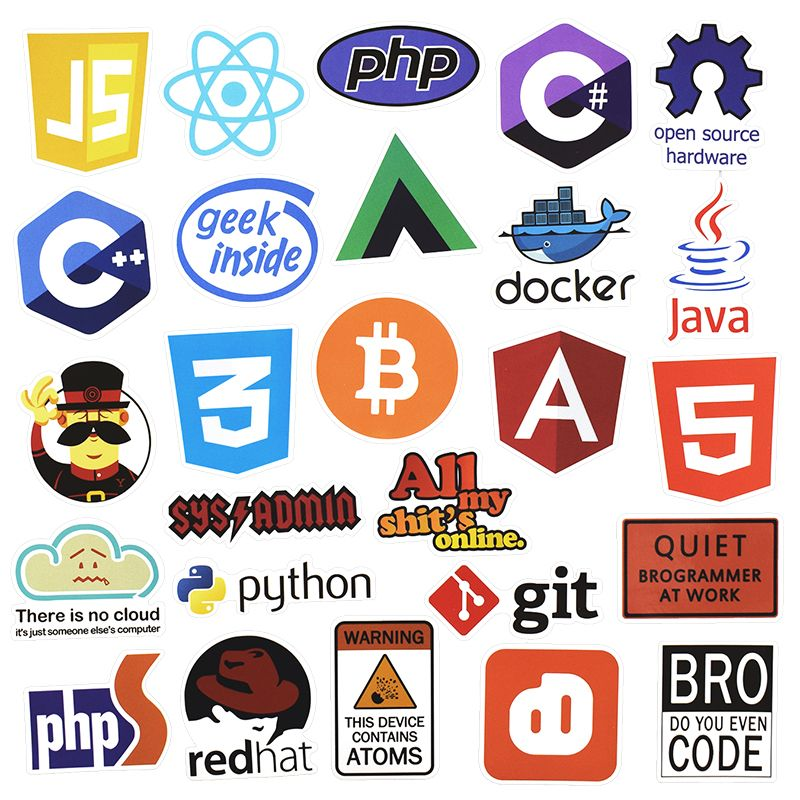
\includegraphics[width=2.5in]{tec_web}
   \caption{Lenguajes, sistemas y tecnologías Web}
   \label{fig:tecnologia_web}
\end{figure}

La mayor parte de la programación está relacionada con la Web y es que la
programación web es muy interesante y amplia, el hecho de que el lenguaje de
programación más popular y usado sea JavaScript, que es el lenguaje que nos
permite interactuar con los navegadores Web, no hace más que confirmar lo
anteriormente mencionado, es por ésto que es importante conocer un poco más la
esencia de la Web en la actualidad.

El objetivo principal de este breve artículo no es solo el de informar qué
tecnologías web son a las que podemos apuntar aprender sino el de instar a
formular proyectos desde ahora ya que el camino de la programación Web implica
adquirir conocimientos, pero más importante aplicarlos y en el camino descubrir
qué nuevos conocimientos podemos y debemos adquirir.

Inicialmente el artículo busca motivar a mis compañeros a involucrarse con el
desarrollo Web y que conozcan las herramientas y tecnologías así como recursos
de aprendizaje a la que todos podemos acceder ya que el Internet es libre, pero
muchas veces no conocemos los recursos y no logramos encontrarlos y
aprovecharlos.

\section{Panorama de la programación Web en el 2018}

Hay que tener en cuenta que en la actualidad el internet funciona de
diferente manera a que lo hacía en los 90's y es que actualmente la Web a
cambiado mucho. Según Sergio Luján Mora, en pocos años, Internet a invadido
casi todos los aspectos de nuestras vidas. Podemos comunicarnos a través de
Internet de distintas formas (correo electrónico, radio y televisión online,
telefonía IP). Podemos comprar diversos productos en Internet (libros,
entradas de cine, ropa). Podemos conocer gente a través de Internet (chat,
foros de discusión, Facebook). Para que ello funcione, hace falta profesionales
especializados en "programación en Internet". En su libro él explica cómo
programar la parte cliente dentro de la arquitectura cliente/servidor. Para
ello enseña HTML y JavaScript principalmente. Sergio Luján menciona que en las
aplicaciones web suelen distinguirse tres niveles: nivel superior que
interacciona con el usuario (el cliente web, normalmente un navegador), el
nivel inferior que proporciona los datos (la base de datos) y el nivel
intermedio que procesa los datos (el servidor web).\cite{SergioLujan2001}.
\newline

La forma en cómo interactuamos con Internet a través de la Web en el 2018
sigue una dirección que se trazó desde inicios del 2000 ya que la web tuvo un
punto de quiebre y los cambios se visualizan en la actualidad ya que ahora se
trata de la Web Social o Web 2.0, donde destacan plataformas como Wikipedia,
Youtube, Facebook, Google, Flickr, Tumblr, Twitter, Instagram, Uber, etc. Y se
tratan de plataformas construidas para la gran masa de usuarios y son éstos los
que crean los contenidos que otros consumen. Según Natalia Vazquez, esta web
está basado en dos princios: \textbf{inteligencia colectiva} que es la suma del
saber de cada uno de los individuos que al compartirse puede dar lugar a una
obra colectiva y la \textbf{arquitectura de la participación} que implica una
nueva forma de construir los sitios web para permitir la participación de la
gran masa de usuarios. La web se convierte entonces en una plataforma de
servicios donde los usuarios asumen una filosofía que supone compartir los
recursos propios a la vez que nos beneficiamos de los ajenos, saldando así una
especie de deuda con la comunidad.\cite{NataliaVazquezWeb2007}.  \newline
\newline

Para construir una página y luego una aplición Web es necesario el conocimiento
de muchas tecnologías y lenguajes de programación. Para empezar podemos citar
un lenguaje de programación que es muy fácil de aprender, emplear y mantener.
Según Marzal Andrés, Python es un un lenguaje de muy alto nivel que permite
expresar algoritmos de forma casi directa, incluso se puede considerar un
``pseudocódigo ejecutable'' y gracias la experiencia en la enseñanza de los
autores del libro ``Introducción a la programación con Python 3'' han concluído
que es un lenguaje particularmente adecuado para el primer punto de contacto
con la programación\cite{IntroPython2008}.
\newline

Actualmente existen muchos lenguajes de programación, cada lenguaje tiene sus
ventajas y desventajas así como su comunidad de programadores que las respalda,
pero los lenguajes de programación manejan la misma lógica, lo que las
diferencia es su forma de manejar la traducción del código, los paradigmas,
y principalmente su sintaxis. Así los lenguajes de
programación nos permiten comunicar instrucciones a las computadoras y lograr
que éstas hagan trabajo por nosotros, es necesario entonces entender la lógica
de programación y hay varias formas de entenderla sin involucrarse con un
lenguaje de programación en específico, la manera más aceptada y es la que
enseña el autor Luis Joyanes en su libro es el
Pseudocódigo\cite{JoyanesProg2008}.
\newline

\begin{figure}[ht]
   \centering
   
\includegraphics[width=2.5in]{git_logo}
   \caption{Sistema de Control de Versiones Git}
   \label{fig:git_sistema}
\end{figure}

El Software Libre es el software que respeta la libertad del usuario y la
solidaridad social de su comunidad. El software que no es libre se llama
Software Privativo porque priva de la libertad a sus usuarios y los mantiene
divididos e impotentes; divididos porque cada uno está prohibido de compartir
con los demás e impotentes porque no tienen el codigo fuente, por lo tanto no
pueden cambiar el programa ni siquiera pueden averiguar lo que realmente hace
el software. El Software Libre brinda al usuario cuatro libertades esenciales:
Libertad 0 que es la libertad de ejecutar el programa como quieras, Libertad 1
que es la libertad de estudiar el código fuente del programa y poder cambiarlo
para que el programa haga lo que quieras, Libertad 2 que es la libertad de
ayudar a tu prójimo de poder hacer copias y distribuirlas a los demás cuando
quieras, Libertad 3 que es la libertad de contribuir a tu comunidad es la
libertad de hacer y distribuir copias de tus versiones cambiadas a los demás
cuando quieras. El desarrollar un programa libre es una contribución a la
sociedad, mas o menos según los detalles técnicos. El Open Source es una
variación práctica de la ideología del Software Libre que no toma en cuenta las
consideraciones éticas de la Libertad pero que en la práctica tienen mucho en
común\cite{StallmanFS2004}.
\newline
\begin{figure}[ht]
   \centering
   
\includegraphics[width=2.5in]{gnu_stallman}
   \caption{Proyecto GNU - Richard Stallman}
   \label{fig:stallman_gnu}
\end{figure}

Las tecnologías web que tienen mayor éxito son las que tienen detrás una
comunidad de desarrolladores grande y activa. Hay comunidades de que usan
lenguajes de programación como JavaScript, Python, Ruby, PHP, etc. Estos
lenguajes de programación son el núcleo del desarrollo de frameworks como
AngularJs de JavaScript, Django de Python, Ruby on Rails de Ruby, o Laravel de
PHP. Según Javier Gutierrez, el framework es una estructura software compuesta
de componentes personalizables e intercambiables para el desarrollo de una
aplicación. En otras palabras, un framework se puede considerar una aplicación
genérica incompleta y configurable a la que podemos añadirle las últimas piezas
para construir una aplicación concreta.\cite{GutierrezFramework}
\newline

La colaboración de la comunidad de programadores para el desarrollo de
proyectos como los frameworks se dan a través de plataformas web por ejemplo
tenemos: GitHub (la más popular), Gitlab, Bitbucket, SourceForge,etc. En éstas
plataformas Web gratuitas y en otras podemos encontrar el código de estos
proyectos, estudiarlos modificarlos y aportar a la comunidad. A continuación
tenemos algunos enlaces a los proyectos de framewoks Web más populares y usados
en el desarrollo de aplicaciones Web: para AngularJS tenemos
\url{https://github.com/angular}, Django \url{https://github.com/django}, Ruby
on Rails \url{https://github.com/rails}, Laravel
\url{https://github.com/laravel}. GitHub también funciona como una red social
de programadores en la que se pueden votar los proyectos y los usuarios. Cada
usuario puede establecer vínculos con otros usuarios y puede seguir lo que
hace. Muchas empresas buscan programadores en esta plataforma hasta el punto de
ser indispensable tener cuenta de GitHub para conseguir trabajo como
programador\cite{LuisGitHub2016}.
\newline

Los proyectos almacenados en GitHub son controlados mediante Git. Git es un
Sistema de Control de Versiones. ¿Qué es un controlador de versiones y por qué
debería importarnos? Un Controlador de versiones (VCS) es un sistema que graba
los cambios realizados en un archivo o conjunto de archivos en el mismo tiempo
que se realizan, así es posible rescatar distintas versiones específicas
después, ésta es una herramienta fundamental para realizar proyectos de
Software. Antes de Git existían los llamados sistemas de control de versiones
locales que lo que hacían era copiar los archivos dentro de otros directorios
de una forma muy común y simple, pero eran propensos a los errores; luego se
usaban los sistemas de control de versiones centralizados que fueron
implementados para permitir el desarrollo colaborativo y fue por mucho años el
estándar para el Control de Versiones ya que ofrecía muchas ventajas frente a
los VCS locales pero presentaban serias desventajas, la más obvia es que el
proyecto y toda su historia se centralizan en un solo punto, así si este
servidor centralizado falla, durante el tiempo que falle nadie podrá colaborar
o guardar los cambios y versiones en las que se estén trabajando y si el disco
duro de la base central de datos se corrompe junto con los respaldos, se pierde
absolutamente toda la historia entera del proyecto excepto la copia que
mantienen localmente los desarrolladores que trabajan en ella, pero la imagen
del proyecto se pierde es por esto que luego nacen los Sistemas de Control de
Versiones Distribuidos (DVCSs) como Git, Mercurial, Baazar o Darcs. Linus
Torvalds es un Ingeniero de Software que es el desarrollador de Linux que es el
núcleo que corre en los sistema GNU/Linux y también es el desarrollador de Git
que nace de la necesidad que tenían los desarrolladores del Kernel de Linux de
trabajar colaborativamente. Así Git nace en el seno del Open Source y
Linux\cite{ScottBenGit2014}.
\newline

A inicios del año 1983, Richard Stallman inició el proyecto GNU que significa
``GNU no es Linux'' y que estaba soportado por la Free Software Fundation con
el objetivo de crear un sistema operativo que sea capaz de ser usado de forma
libre respetando los lineamientos de la FSF con sus cuatro libertades. Richard
y su equipo consiguieron todas las herramientas necesarias para hacer que un
computador funciones con software libre, pero hacía falta el núcleo que
gestione los recursos y tareas del computador, para eso Linus Torvalds estaba
desarrolando en paralelo un Kernel basado en Minix que era una versión simple
de UNIX que tenía por finalidad la educación. Cuando Linus libera su Kernel al
que denomina Linux, que solo, no era capaz de hacer nada, se integra con todas
las herramientas creadas por el proyecto GNU y logran instalar el primer
Sistema Operativo en un computador usando solamente software Libre.
Actualmente Google corre miles de miles de servidores Linux que soporta su
tecnología de búsqueda, incluso su sistema operativo Android corre el kernel
Linux. Facebook construye y desarrolla su sitio web usando todo lo relacionado
con LAMP stack (Linux, Apache, Web server, MySQL database y PHP). Las
organizaciones finalciales que tienen trillones de dólares corriendo sobre la
velocidad y seguridad de sus sitemas operativos que dependen fuertemente de
Linux\cite{ChrisNegusLinux2005}.
\newline

\section{Rutas de aprendizaje}
Si se analiza, en la actualidad hay dos mundos que coexisten en el desarrollo
web: Fronted y Backend.\\
Entonces al ingresar a la programación Web se puede acceder a dos rutas de
aprendizaje: Fronted o Backend.\\

Si aprendes Fronted serás un Fronted Developer. 
¿Qué significa ser Fronted Developer? Significa ser un desarrollador capaz de
convertir en real un diseño de UX/UI (User Experiencie / Use Interface) y
programar la reacción ante la interacción que pueda tener el usuario dentro de
la web y además conocer bien cómo recibir y enviar datos del servidor
(backend). Fronted es más rápido de aprender que Backend, pero no
necesariamente lo más fácil.\\

Si aprendes Backend serás un Backend Developer.
Un desarollador Backend es un programador que trabaja del lado del servidor.
Permitiendo que todo lo que vemos cuando interactuamos con una aplicación o
sitio web, funcione. Dicho de una forma más informal, es el que trabaja detrás
del escenario, moviendo los hilos para que todo salga bien.
Ahora hay una ruta que se abre si eliges el camino del Backend y es la del
DevOps que viene de Development Operations. ¿Qué es DevOps? Es un camino para
implementar Software con esfuerzo y responsabilidad compartida, así un DevOps
Developer conoce el cómo implementar un software, su ciclo de vida y
mantenimiento, actualmente es un cargo de moda que se requiere mucho en la
industria y profesionales con éste perfil tienen muchos beneficios
financieros.\\


\subsection{Fronted}
Existen tres tecnologías pilares en la parte Fronted de la programación Web,
tenemos: HTML, CSS, JavaScript.\\
HTML es un lenguaje de marcado para la elaboración de páginas Web. Es un
estándar que está a cargo del \textit{World Wide Consortium} (W3C). HTML
permite organizar la información, para eso usa etiquetas, atributos y valores.
En HTML5 se cuenta con etiquetas que dan significado a una porción de
información útil para buscadores como Google, así Google va directo a la
información contenida dentro de una etiqueta y la interpreta de forma
inteligente, esto le sirve por ejemplo para clasificar las páginas web por su
contenido, encontrar imágenes y videos, y destacar la información importante
que ofrece la página al momento de hacer una búsqueda, ésto se denomina Web
semántica.\\
Una etiqueta se inicia con el signo ``$<$'' y se finaliza con ``$>$''. Dentro
de una etiqueta va su nombre y también pueden ir atributos que a su vez pueden
tener valores.\\
Podemos ver en la imagen ~\ref{fig:html_etiquetado} un ejemplo de cómo se vería
un esquema html básico. HTML se puede aprender gratis visitando la siguiente
documentación \cite{HTMLw3:2018:online}.

\begin{figure}[ht]
   \centering
   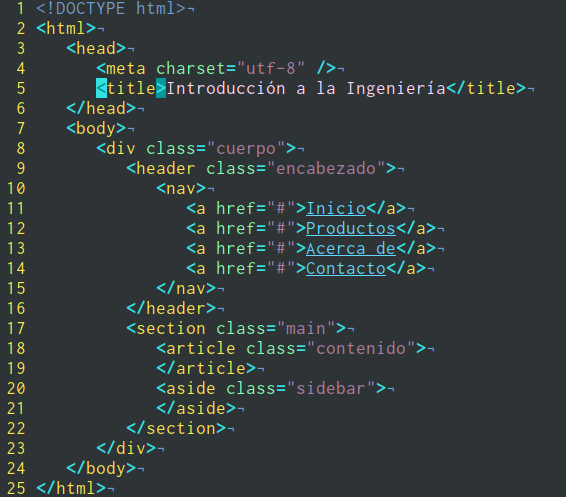
\includegraphics[width=2.5in]{html}
   \caption{Etiquetado en HTML}
   \label{fig:html_etiquetado}
\end{figure}

Al inicio todo el mundo Web estaba hecho solo con HTML; sin embargo dar estilo
a una página Web para hacerla ver más atractiva y organizada era muy complicado
de hacer solo usando HTML, es por eso que surge CSS. Actualmente ya no se da
estilo a una página web usando HTML ya que éste se dedica solo al estructurado
de la información.
CSS (Cascading Style Sheets) es un lenguaje de diseño gráfico para definir y
crear la presentación de un documento estructurado como HTML. CSS funciona con
el uso de selectores (de etiquetas HTML, id o clases), propiedades que adoptan
valores como podemos ver en la imagen ~\ref{fig:css_ejemplo}.\\
Es necesario practicar bastante el lenguaje CSS realizando muchos proyectos
hasta que se llegue a un punto en el que se puede realizar un diseño y
maquetarlo ``en términos de CSS''; también es recomendable relacionarse con
diseñadores, hablar de diseño, entender el diseño hasta que se adquiera un
gusto de diseñador, ésto último no es necesario pero si marca diferencia al
momento de crear interfaces de usuario amigables, atractivos que otorguen una
experiencia positiva al usuario.\\
CSS por otro lado es muy importante en la actualidad porque permite un
desarrollo con el llamado ``\textit{Responsive Design}'', que hace que nuestro
diseño se adapte a diferentes dispositivos con diferente tamaño de pantalla.
Así con el uso de modulos como: \textit{Media query}, \textit{Flexbox},
\textit{Grid}, etc. Podemos definir una disposición en una pantalla de 48
pulgadas y otra en un dispositivo Smartphone, el diseño se adapta.\\

HTML y CSS no son lenguajes de programación como lo es JavaScript. JavaScript
es un lenguaje de programación que nos permite interactuar con el navegador.
Nos brinda la posibilidad de otorgarle a nuestra página web interactividad. Los
paneles desplegables, las ventanas emergentes, los slides o imagenes que se
mueven, etc.\\
Si has elegido el camino del Fronted, el primer lenguaje recomendable de
aprender es JavaScript, porque es un lenguaje fácil y muy versátil, hoy en día
está en casi todos lados: Sistemas Operativos, Desarrollo móvil, servidores de
Internet, base de datos, plataformas de juegos, administración de sistemas,
tanto Linux como Windows y si nos centramos en la web incluso se puede usar
JavaScript como el único lenguaje de programación, desde el cliente hasta el
servidor pasando por la base de datos. El famos stack MEAN (MongoDB + Express +
AngularJS + NodeJS) utiliza JavaScript como único lenguaje.
Puedes visitar la siguiente documentación para estudiar JavaScript, que por
cierto no tiene nada que ver con Java excepto el nombre
\cite{JavaScriptw3:2018:online} \cite{PluralsightJavaScript:2018:online}.
Una vez ya aprendiste lo básico de JavaScript puedes iniciar con el uso de
Frameworks de JavaScript como AngularJS si te gusta Java o React JS si
prefieres PHP o últimamente se está popularizando más VueJS que es un framework
enteramente mantenido por la comunidad a diferencia de AngularJS que es
mantenido por Google o React que es mantenido por Facebook.

\begin{figure}[ht]
   \centering
   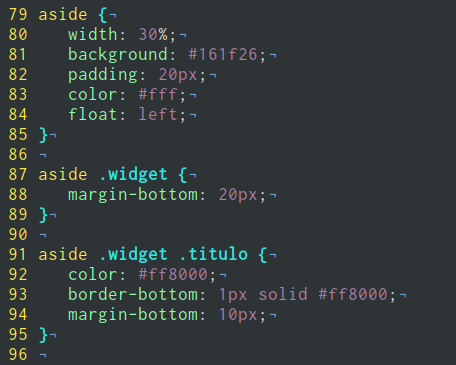
\includegraphics[width=2.5in]{css_ejemplo}
   \caption{Selectores y propiedades en CSS}
   \label{fig:css_ejemplo}
\end{figure}























\section{Requerimientos necesarios}
Al formarse como programador Web es necesario escoger una ruta, ya que para
dedicarse a esta rama de la informática incluso hay que especializarse. Se
puede elegir entre dos caminos o rutas: Fronted y Backend, pero antes de entrar
en detalle de estas dos ruta es necesario conocer algunas herramientas y
fundamentos que nos ayudarán sin importar cual sea el camino que hayamos
elegido.
\subsection{Git - Sistema de control de versiones}
\cite{pascual199012}\cite{mycite2016}\cite{Chavez-Campos2016}\cite{webdev:2018:online}\cite{SergioLujan2001}\cite{NataliaVazquezWeb2007}\cite{WebDev:2018:online}\cite{ScottBenGit2014}\cite{Ssh:2018:online}\cite{HTTP:2018:online}\cite{HTTPS:2018:online}\cite{ChrisNegusLinux2005}\cite{JoyanesProg2008}\cite{GuidesGitHub:2018:online}\cite{HTMLw3:2018:online}\cite{PluralsightJavaScript:2018:online}\cite{JavaScriptw3:2018:online}\cite{PythonTuto:2018:online}\cite{IntroPython2008}


\printbibliography
\end{document}
